\documentclass{article}
% For math environments
\usepackage{amsmath, amsfonts}
% For links
\usepackage[hidelinks]{hyperref}
% So space it put between paragraphs
\usepackage{parskip}
% For figures
\usepackage{tikz}
% Set the margins to not be ridiculous
\usepackage[margin=0.75in]{geometry}
% For multiple columns
\usepackage{multicol}
% For controlling enum/itemize spacing and indentation
\usepackage{enumitem}

% For tikz plots
\usepackage{pgfplots}
% This isn't needed but avoids a compiler warning
\pgfplotsset{compat=1.16}

% Allow multi-line equations to be broken across pages
\allowdisplaybreaks

% Use @ as a letter
\makeatletter

% Scale down all tikz coordinates while maintaining font size
\tikzset{every picture/.style={scale=0.45, every picture/.style={}}}


% Macros
% Monospace code
\def\code#1{\texttt{#1}}

% Greek letters
\def\a{\alpha}
\def\b{\beta}
\def\g{\gamma}
\def\d{\delta}
\def\D{\Delta}

% Some common sets
\def\es{\varnothing}
\def\ints{{\mathbb{Z}}}

% Commands that make life easier
\newcommand\gath[1]{\begin{gather} #1 \end{gather}}
\newcommand\gaths[1]{\begin{gather*} #1 \end{gather*}}
\newcommand\ali[1]{\begin{align} #1 \end{align}}
\newcommand\parens[1]{\left( #1 \right)}
\newcommand\squares[1]{\left[ #1 \right]}
\newcommand\braces[1]{\left\{ #1 \right\}}
\newcommand\angles[1]{\left\langle #1 \right\rangle}
\newcommand\deriv[2]{\frac{d #1}{d #2}}
\newcommand\abs[1]{\left| #1 \right|}
\newcommand\floor[1]{\left\lfloor #1 \right\rfloor}
\newcommand\ceil[1]{\left\lceil #1 \right\rceil}
\DeclareMathOperator{\lcm}{lcm}
\def\non{\nonumber \\}
\newcommand\unit[1]{~\mathrm{#1}}
\newcommand\combos[2]{{}_{#1}C_{#2}}

% Set stuff
\def\ss{\subseteq}

% Multiline equation space
\def\mlesp{\hspace{1.2cm}}

% For grid diagrams
\newcommand\gridbox[3]{\draw (#1,#2) rectangle (#1+1,#2+1) node[pos=.5] {#3};}
\newcommand\gridboxh[3]{\draw[fill=red!20] (#1,#2) rectangle (#1+1,#2+1) node[pos=.5] {#3};}
\newcommand\gridboxb[3]{\draw[fill=black] (#1,#2) rectangle (#1+1,#2+1) node[pos=.5] {#3};}
\newcommand\gridsym[3]{\node at (#1+0.5,#2+0.5) {$#3$};}
\newcommand\gridblank[2]{\filldraw[draw=gray, color=gray] (#1,#2) rectangle (#1+1,#2+1);}
\newcommand\gridcirc[2]{\draw (#1 + 0.5,#2 + 0.5) circle (0.25);}
\newcommand\cwlab[3]{
  \def\dd{0.15}
  \draw (#1 + \dd - 0.03, #2 + 1 - \dd) node {\scriptsize #3};
}

\def\bbw{3.5}
\def\bbh{2}
\newcommand\bigbox[3]{\draw (#1*\bbw,#2*\bbh) rectangle (#1*\bbw+\bbw,#2*\bbh+\bbh) node[pos=.5] {#3};}
\newcommand\bbtextr[3]{\node[right] at (#1*\bbw,#2*\bbh+0.5*\bbh) {#3};}
\newcommand\bbtextb[3]{\node[align=center] at (#1*\bbw+0.5*\bbw,#2*\bbh+0.5*\bbh) {#3};}

% Box puzzle stock answer
\newcommand\boxans[1]{
  Logic was used to deduce the solution:

  #1

  This was verified using Python as well as shown to be unique with a brute force approach.
}

% Standard crossnumber grid
\newcommand\crossnumstd[9]{
  \begin{center}
    \begin{tikzpicture}[scale=2]
      \gridbox{0}{2}{#1}
      \gridbox{1}{2}{#2}
      \gridbox{2}{2}{#3}
      \gridbox{0}{1}{#4}
      \gridbox{1}{1}{#5}
      \gridbox{2}{1}{#6}
      \gridbox{0}{0}{#7}
      \gridbox{1}{0}{#8}
      \gridbox{2}{0}{#9}

      % Labels
      \cwlab{0}{2}{1}
      \cwlab{1}{2}{2}
      \cwlab{2}{2}{3}
      \cwlab{0}{1}{4}
      \cwlab{0}{0}{5}
    \end{tikzpicture}
  \end{center}
}

% Multiple numbers
\newcommand\mn[1]{$#1$'s}

% Commands for problems
\newcommand\problem[4]{
\section*{#1}

\textbf{Question:} #3

\textbf{Answer:} #2

\textbf{Explanation:} #4
}
\newcommand\aproblem[4]{\problem{Dec #1}{#2}{#3}{#4}}
\newcommand\cproblem[4]{\problem{Problem #1}{#2}{#3}{#4}}

\newcommand\xref@advent[2]{#1 Advent, Dec~#2 problem}
\newcommand\xref@card[2]{#1 Christmas Card, Problem #2}

% For answered verified with Python
\newcommand{\verified}{This was verified with a brute-force Python program.}

\def\advent@xxi@i{
  The geometric mean of a set of $n$ numbers can be computed by multiplying together all the numbers then computing the $n$th root of the result.

  The factors of $4$ are $1$, $2$ and $4$. The geometric mean of these is 2.

  The factors of $6$ are $1$, $2$, $3$, and $6$. The geometric mean of these is $\sqrt{6}$.

  The geometric mean of all the factors of today's number is $22$.
}

\def\advent@xxi@ii{
  The number $7n$ has $37$ factors (including $1$ and the number itself).
  How many factors does $8n$ have?
}

\def\advent@xxi@iii{
  If you write out the numbers from $1$ to $1000$ (inclusive), how many times will you write the digit $0$?
}

\def\advent@xxi@iv{
  Put the digits $1$ to $9$ (using each digit exactly once) in the boxes so that the sums are correct.
  The sums should be read left to right and top to bottom ignoring the usual order of operations.
  For example, $4 + 3 \times 2$ is $14$, not $10$.
  Today's number is the product of the numbers in the red boxes.

  \grid@advent@xxi@iv{}{}{}{}{}{}{}{}{}
}

\def\advent@xxi@v{
  How many different isosceles triangles are there whose perimeter is $50$ units, and whose area is an integer number of units squared?

  (Two triangles that are rotations, reflections and translations of each other are counted as the same triangle. Triangles with an area of 0 should not be counted.)
}

\def\advent@xxi@vi{
  When $12345$ is divided by today's number, the remainder is $205$.
  When $6789$ is divided by today's number, the remainder is $112$.
}

\newcommand\dec@ai{0.30901699437494745}
\newcommand\dec@aii{0.8090169943749475}
\newcommand\dec@bi{0.5877852522924731}
\newcommand\dec@bii{0.9510565162951535}
\newcommand\decagon[5]{
  \def\ai{\dec@ai*#3+#1}
  \def\aii{\dec@aii*#3+#1}
  \def\bi{\dec@bi*#3+#2}
  \def\bii{\dec@bii*#3+#2}
  \draw (#3+#1, #2) -- (\aii, \bi) -- (\ai, \bii) -- (-\ai, \bii) -- (-\aii, \bi) -- (-#3+#1, #2) -- (-\aii, -\bi) -- (-\ai, -\bii) -- (\ai, -\bii) -- (\aii, -\bi) -- cycle;
  \fill[fill=red] (-\ai, -\bii) -- (#4*#3+#1, #5*#3+#2) -- (\ai, -\bii) -- cycle;
}
\def\advent@xxi@vii{
  The picture below shows eight regular decagons.
  In each decagon, a red triangle has been drawn with vertices at three of the vertices of the decagon.

  \begin{center}
    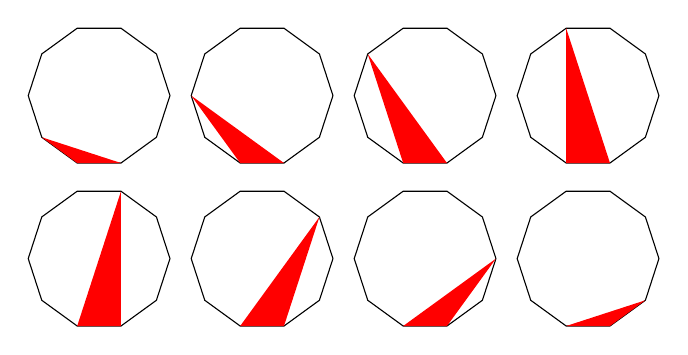
\begin{tikzpicture}
      \def\dr{2}
      \def\spc{2.3*\dr}

      \decagon{0*\spc}{\spc}{\dr}{-\dec@aii}{-\dec@bi}
      \decagon{1*\spc}{\spc}{\dr}{-1}{0}
      \decagon{2*\spc}{\spc}{\dr}{-\dec@aii}{\dec@bi}
      \decagon{3*\spc}{\spc}{\dr}{-\dec@ai}{\dec@bii}

      \decagon{0*\spc}{0}{\dr}{\dec@ai}{\dec@bii}
      \decagon{1*\spc}{0}{\dr}{\dec@aii}{\dec@bi}
      \decagon{2*\spc}{0}{\dr}{1}{0}
      \decagon{3*\spc}{0}{\dr}{\dec@aii}{-\dec@bi}
    \end{tikzpicture}
  \end{center}

  The area of each decagon is $240$.
  What is the total area of all the red triangles?
}

\def\advent@xxi@viii{
  The sum of three integers is $51$.
  The product of the same three integers is $836$. What is the product of largest integer and the second-largest integer?
}

\def\advent@xxi@ix{
  Eve writes down a sequence of consecutive positive integers (she writes more than one number).
  The sum of the numbers Eve has written down is $844$.
  Today's number is the smallest integer that Eve has written down.
}

\def\advent@xxi@x{
  Put the digits $1$ to $9$ (using each digit exactly once) in the boxes so that the sums are correct.
  Today's number is the largest number you can make using the digits in the red boxes.

  \grid@advent@xxi@x{}{}{}{}{}{}{}{}{}
}

\def\advent@xxi@xi{
  The integers are written in a triangle as shown below:
  \begin{center}
    \begin{tabular}{ccccccc}
         &    &    & 1    &    &    &    \\
         &    & 2  & 3    & 4  &    &    \\
         & 5  & 6  & 7    & 8  & 9  &    \\
      10 & 11 & 12 & 13   & 14 & 15 & 16 \\
         &    &    & etc. &    &    &
    \end{tabular}
  \end{center}
  Today's number appears directly above the number $750$ in the triangle of integers.
}

\def\advent@xxi@abgrid{
  \begin{center}
    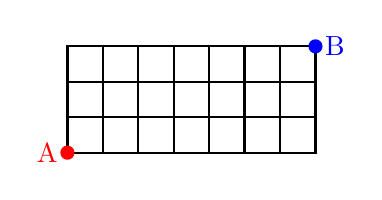
\begin{tikzpicture}
      \def\gs{1}
      % Grid
      \foreach \i in {0,...,6}{
          \foreach \j in {0,...,2}{
              \draw[thick] (\i * \gs, \j * \gs) rectangle (\i * \gs + \gs, \j * \gs + \gs);
            }
        }
      % Points
      \fill[color=red] (0, 0) circle (0.2) node[color=red,left] {A};
      \fill[color=blue] (7*\gs, 3*\gs) circle (0.2) node[color=blue,right] {B};
    \end{tikzpicture}
  \end{center}
}
\def\advent@xxi@xii{
  You start at the point marked A in the picture below. You want to get to the point marked B.
  You may travel \textbf{to the right} or \textbf{upwards} along the black lines.

  \advent@xxi@abgrid

  Today's number is the total number of possible routes to get from A to B.
}

\def\advent@xxi@xiii{
  The diagram below shows three circles and two triangles.
  The three circles all meet at one point.
  The vertices of the smaller red triangle are at the centers of the circles.
  The lines connecting the vertices of the larger blue triangle to the point where all three circles meet are diameters of the three circles.

  \begin{center}
    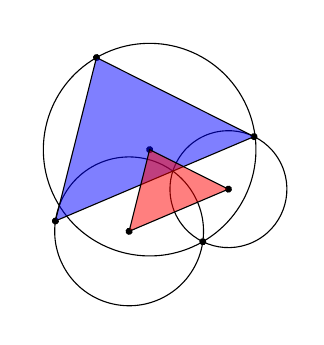
\begin{tikzpicture}[rotate=30,transform shape]
      \def\bcr{3}
      \def\scr{0.55*\bcr}
      \def\sca{34}
      \def\mcr{0.7*\bcr}
      \def\mca{142}
      \def\pr{0.1}

      % Circles
      \draw (0, \bcr) circle (\bcr);
      \draw (\sca: \scr) circle (\scr);
      \draw (\mca: \mcr) circle (\mcr);

      % Points
      \fill (0, 0) circle (\pr);
      \fill (0, \bcr) circle (\pr);
      \fill (0, 2*\bcr) circle (\pr);
      \fill (\sca: \scr) circle (\pr);
      \fill (\sca: 2*\scr) circle (\pr);
      \fill (\mca: \mcr) circle (\pr);
      \fill (\mca: 2*\mcr) circle (\pr);

      % Triangles
      \draw[fill=blue,fill opacity=0.5] (\mca: 2*\mcr) -- (0, 2*\bcr) -- (\sca: 2*\scr) -- cycle;
      \draw[fill=red,fill opacity=0.5] (\mca: \mcr) -- (0, \bcr) -- (\sca: \scr) -- cycle;
    \end{tikzpicture}
  \end{center}

  The area of the smaller red triangle is $226$.
  What is the area of the larger blue triangle?
}

\def\advent@xxi@xiv{
  You start at the point marked A in the picture below.
  You want to get to the point marked B.
  You may travel \textbf{to the right}, \textbf{upwards}, or \textbf{to the left} along the black lines, but you cannot pass along the same line segment more than once.

  \advent@xxi@abgrid

  Today's number is the total number of possible routes to get from A to B.
}

\newcommand\pyramid@advent@xxi@xvi[6]{
  \begin{center}
    \begin{tabular}{cccccc}
      (row 1) &    &    & #1   &    &    \\
      (row 2) &    & #2 &      & #3 &    \\
      (row 3) & #4 &    & #5   &    & #6 \\
              &    &    & etc. &    &
    \end{tabular}
  \end{center}
}
\def\advent@xxi@xv{
  The odd numbers are written in a pyramid.

  \pyramid@advent@xxi@xvi{1}{3}{5}{7}{9}{11}

  What is the mean of the numbers in the 19th row?
}

\newcommand\grid@advent@xxi@xvi[9]{
  \begin{center}
    \begin{tikzpicture}[scale=2]
      \gridbox{0}{2}{#1}
      \gridbox{1}{2}{#2}
      \gridbox{2}{2}{#3}
      \gridbox{0}{1}{#4}
      \gridbox{1}{1}{#5}
      \gridbox{2}{1}{#6}
      \gridbox{0}{0}{#7}
      \gridbox{1}{0}{#8}
      \gridbox{2}{0}{#9}

      % Labels
      \cwlab{0}{2}{1}
      \cwlab{1}{2}{2}
      \cwlab{2}{2}{3}
      \cwlab{0}{1}{4}
      \cwlab{0}{0}{5}
    \end{tikzpicture}
  \end{center}
}
\def\advent@xxi@xvi{
  Each clue in this crossnumber is formed of two parts connected by a logical connective: AND means that both parts are true; NAND means that at most one part is true; OR means that at least one part is true; NOR means that neither part is true; XOR means that exactly one part is true; XNOR means that either both parts are false or both parts are true.
  No number starts with $0$.

  \begin{multicols}{2}
    \grid@advent@xxi@xvi{}{}{}{}{}{}{}{}{}

    \columnbreak

    \begin{enumerate}
      \item \textbf{1A} is a palindrome XNOR \textbf{1D} is a palindrome.
      \item \textbf{1A} is greater than $350$ NOR \textbf{1D} is less than $150$.
      \item \textbf{3D} is odd NAND \textbf{4A} and \textbf{2D} are equal.
      \item \textbf{3D} is prime XOR \textbf{5A} is odd.
      \item \textbf{4A} is a cube AND \textbf{2D} is a cube.
      \item The sum of the digits of \textbf{3D} is $2$ OR the sum of the digits of \textbf{5A} is $5$.
      \item Today's number is \textbf{1D}.
    \end{enumerate}
  \end{multicols}
}

\def\advent@xxi@xvii{
  The digital product of a number is computed by multiplying together all of its digits. For example, the digital product of $6273$ is $252$.

  Today's number is the smallest number whose digital product is $252$.
}

\def\advent@xxi@xviii{
  Put the digits $1$ to $9$ (using each digit exactly once) in the boxes so that the sums are correct.
  The sums should be read left to right and top to bottom ignoring the usual order of operations.
  For example, $4 + 3 \times 2$ is $14$, not $10$.
  Today's number is the product of the numbers in the red boxes.

  \grid@advent@xxi@xviii{}{}{}{}{}{}{}{}{}
}

\def\advent@xxi@xix{
  The equation $352x^3 - 528x^2 + 90 = 0$ has three distinct real-valued solutions.

  Today's number is the number of integers $a$ such that the equation $352x^3 - 528x^2 + a = 0$ has three distinct real-valued solutions.
}

\def\advent@xxi@xx{
  What is the area of the largest area triangle that has one side of length $32$ and one side of length $19$?
}

\newcommand\grid@advent@xxi@xxi[9]{
  \begin{center}
    \begin{tikzpicture}
      \bigbox{0}{3}{#1}
      \bigbox{1}{3}{#2}
      \bigbox{2}{3}{#3}
      \bbtextr{3}{3}{\textbf{today's number}}

      \bigbox{0}{2}{#4}
      \bigbox{1}{2}{#5}
      \bigbox{2}{2}{#6}
      \bbtextr{3}{2}{prime}

      \bigbox{0}{1}{#7}
      \bigbox{1}{1}{#8}
      \bigbox{2}{1}{#9}
      \bbtextr{3}{1}{square}

      \bbtextb{0}{0}{cube}
      \bbtextb{1}{0}{odd}
      \bbtextb{2}{0}{multiple\\of $11$}
    \end{tikzpicture}
  \end{center}
}
\def\advent@xxi@xxi{
  Arrange the digits $1$–$9$ (using each digit exactly once) so that the three digit number in: the middle row is a prime number; the bottom row is a square number; the left column is a cube number; the middle column is an odd number; the right column is a multiple of $11$.
  The $3$-digit number in the first row is today's number.

  \grid@advent@xxi@xxi{}{}{}{}{}{}{}{}{}
}

\def\advent@xxi@xxii{
  There are $12$ ways of placing $2$ tokens on a $2 \times 4$ grid so that no two tokens are next to each other horizontally, vertically or diagonally:

  \begin{center}
    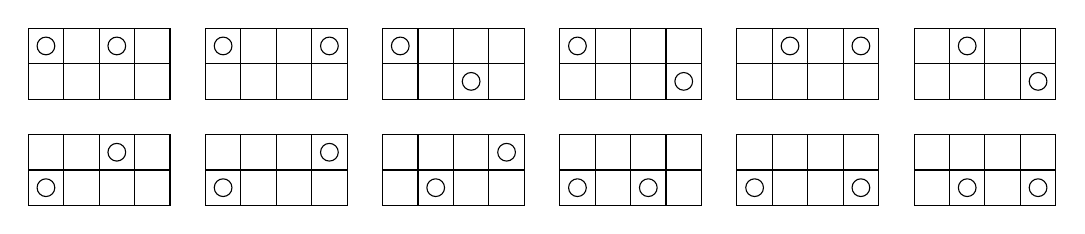
\begin{tikzpicture}
      % Draw all the grids
      \foreach \gi in {0,1}{
          \foreach \gj in {0,...,5}{
              \foreach \i in {0,1}{
                  \foreach \j in {0,...,3}{
                      \gridbox{5*\gj + \j}{3*\gi + \i}{}
                    }
                }
            }
        }

      % Place token circles
      \gridcirc{0}{4}
      \gridcirc{2}{4}
      \gridcirc{5}{4}
      \gridcirc{8}{4}
      \gridcirc{10}{4}
      \gridcirc{12}{3}
      \gridcirc{15}{4}
      \gridcirc{18}{3}
      \gridcirc{21}{4}
      \gridcirc{23}{4}
      \gridcirc{26}{4}
      \gridcirc{28}{3}
      \gridcirc{0}{0}
      \gridcirc{2}{1}
      \gridcirc{5}{0}
      \gridcirc{8}{1}
      \gridcirc{11}{0}
      \gridcirc{13}{1}
      \gridcirc{15}{0}
      \gridcirc{17}{0}
      \gridcirc{20}{0}
      \gridcirc{23}{0}
      \gridcirc{26}{0}
      \gridcirc{28}{0}
    \end{tikzpicture}
  \end{center}

  Today's number is the number of ways of placing $2$ tokens on a $2 \times 21$ grid so that no two tokens are next to each other horizontally, vertically or diagonally.
}

\def\advent@xxi@xxiii{
  I draw the parabola $y = x^2$ and mark points on the parabola at $x = 17$ and $x = -6$.
  I then draw a straight line connecting these two points.

  At which value of $y$ does this line intercept the $y$-axis?
}

\def\advent@xxi@xxiv{
  The digital product of a number is computed by multiplying together all of its digits.
  For example, the digital product of $1522$ is $20$.

  How many $12$-digit numbers are there whose digital product is $20$?
}

\def\card@xxi@i{
  What is the sum of all the odd integers between $0$ and $30$?
}

\def\card@xxi@ii{
  What is the sum of all the odd integers between $0$ and $5668$?
}

\def\card@xxi@iii{
  What is the smallest integer with a digital sum of $28$ and a digital product of $10000$?
}

\def\card@xxi@iv{
  What is the smallest integer with a digital sum of $41$ and a digital product of $432000$?
}

\def\card@xxi@v{
  What is the area of the largest area dodecagon that will fit inside a circle with area $111185 \pi$?
}

\def\card@xxi@vi{
  What is the area of the largest area heptagon that will fit inside a semicircle with area $115185 \pi$?
}

\def\card@xxi@vii{
  How many terms are there in the (simplified) expansion of $(x + y + z)^2$?
}

\def\card@xxi@viii{
  How many terms are there in the (simplified) expansion of $(x + y + z)^{41172}$?
}

\def\card@xxi@ix{
  What is the largest integer that cannot be written as $4a + 5b$ for non-negative integers $a$ and $b$?
}

\def\card@xxi@x{
  What is the largest integer that cannot be written as $83409a + 66608b$ for non-negative integers $a$ and $b$?
}

\def\card@xxi@xi{
  How many positive integers are there below $100$ whose digits are all non-zero and different?
}

\def\card@xxi@xii{
  How many positive integers are there whose digits are all non-zero and different?
}

\def\card@xxi@xiii{
  What is the only integer for which taking the geometric mean of all its factors (including $1$ and the number itself) gives $2$?
}

\def\card@xxi@xiv{
  What is the only integer for which taking the geometric mean of all its factors (including $1$ and the number itself) gives $25$?
}


\begin{document}

\title{Matthew Scroggs 2025 Christmas Card Solutions}
\author{Dan Whitman}
\date{}

\maketitle

Link to the online card: \href{https://www.mscroggs.co.uk/blog/121}{https://www.mscroggs.co.uk/blog/121}

\cproblem{1}{36}{\card@xxv@i}{
  Suppose that $N$ is an even number, and we are interested in the sum of all integers between $0$ and $N$, and denote this by $S(N)$.
  Odd numbers of course can have the form $n = 2k-1$.
  The first odd number after $0$ is obviously $1 = 2 \cdot 1 - 1$.
  The last odd number before $N$ is then $N - 1$ so that
  \gath{
    2k - 1 = N -1 \non
    2k = N \non
    k = \frac{N}{2}.
  }
  Therefore, we have
  \ali{
    S(N) &= \sum_{k=1}^{N/2} (2k-1) = 2 \sum_{k=1}^{N/2} k - \sum_{k=1}^{N/2} 1 \non
    &= 2 \frac{\frac{N}{2}\parens{\frac{N}{2} + 1}}{2} - \parens{\frac{N}{2} - 1 + 1} \non
    &= \frac{N(N+2)}{4}  - \frac{2N}{4} \non
    &= \frac{N(N + 2 - 2)}{4} \non
    &= \frac{N^2}{4}.
  }
  This results in our answer $S(12) = 12^2 / 4 = 36$.
  \verified{}
}

\cproblem{2}{493817284}{\card@xxv@ii}{
  As we know from the previous problem that the sum is
  \gath{
    S(N) = \frac{N^2}{4}
  }
  so that our answer here is $S(44444) = 493817284$.
}

\cproblem{3}{13}{\card@xxv@iii}{
  This can be expressed as the system of modulo congruences:
  \ali{
    x &= 1 \pmod{3} \non
    x &= 1 \pmod{4}.
  }
  Then by the Chinese remainder theorem, this has a unique solution modulo $N = 3 \cdot 4 = 12$ since $3$ and $4$ are coprime.
  Now, clearly $x = 1$ is a solution, but presumably everyone must get at least one bauble, so that next smallest solution is $x = N + 1 = 13$, which must be our answer.
  \verified{}
}

\cproblem{4}{2521}{\card@xxv@iv}{
  Just like the previous problem, this can clearly be expressed as the following system of modulo congruences:
  \ali{
    x &= 1 \pmod{2} \non
    x &= 1 \pmod{3} \non
    x &= 1 \pmod{4} \non
    x &= 1 \pmod{5} \non
    x &= 1 \pmod{6} \non
    x &= 1 \pmod{7} \non
    x &= 1 \pmod{8} \non
    x &= 1 \pmod{9}.
  }
  In this more general case (relative tothe previous problem) the Chinese remainder theorem says that the solution is unique modulo $N = \lcm(2, 3, 4, 5, 6, 7, 8, 9) = 2520$.
  Since again $x = 1$ is a solution and everyone should get at least one bauble, the next smallest solution and our answer is $x = N + 1 = 2521$.
  \verified{}
}

\cproblem{5}{123}{\card@xxv@v}{
  The answer is clearly simply $123$, which is intuitively obvious since we simply select the smallest nonzero digit that has not been used yet, starting at the hundreds place and moving right.
  \verified{}
}

\cproblem{6}{986409}{\card@xxv@vi}{
  This is a permutation problem.
  For the first digit we have 9 choices (i.e. the digits 1 through 9), 8 for the second digit, and 7 for the third, hence our answer is $9 \cdot 8 \cdot 7 = 504$.
  \verified{}
}

\cproblem{7}{11}{\card@xxv@vii}{
  First we solve a more general problem: suppose the same Christmas game except that you can either win $a > 0$ points or $b > 0$ points.
  Hence, for this specific problem, it will be that $a = 4$ and $b = 5$.
  Clearly, since we can have any number of turns, any game will end on some score $c$ where
  \gath{
    ax + by = c. \label{eqn:07:orig}
  }
  This is a linear Diophantine equation where of course $x$ and $y$ must be non-negative integers.
  Call a solution $(x, y)$ \emph{valid} if both $x \geq 0$ and $y \geq 0$ but they are not both zero, since that would result in a score of zero.
  For a general linear Diophantine in which $x$ and $y$ can be \emph{any} integers, a necessary and sufficient condition for the existence of a solution is that $d = \gcd(a, b)$ divides $c$.
  The base integer solution $(x_0, y_0)$ to
  \gath{
    a x_0 + b y_0 = d
  }
  can be found using the \href{https://en.wikipedia.org/wiki/Extended_Euclidean_algorithm}{extended Euclidean algorithm}, which will not be reviewed here.
  So assume that we have that solution in hand.
  We then have that
  \gath{
    a x_0 + b y_0 = d \non
    \frac{a x_0}{d} + \frac{b y_0}{d} = \frac{d}{d} = 1 \non
    \frac{c a x_0}{d} + \frac{c b y_0}{d} = c \non
    a \frac{c x_0}{d} + b \frac{c y_0}{d} = c
  }
  so that $(c x_0/d, c y_0/d)$ is a base solution to our original equation \eqref{eqn:07:orig}.
  Then there are an infinite number of solutions $(x, y)$ to \eqref{eqn:07:orig}:
  \ali{
    x &= \frac{c x_0}{d} + \frac{b t}{d} \non
    y &= \frac{c y_0}{d} - \frac{a t}{d} \label{eqn:07:xy}
  }
  for all $t \in \ints$.
  We are of course actually interested in only valid solutions.
  In this case, $d$ dividing $c$ is still a necessary condition, but not a sufficient one.
  Note that, if $a$ and $b$ are coprime, then $d = 1$, which of course divides every $c$, so that any $c$ will potentially have solutions.
  If $a$ and $b$ were not coprime then there would be an infinite number of $c$ such that $d$ does not divide $c$, and hence an infnite number of impossible scores.
  For valid solutions then, from \eqref{eqn:07:xy}, we must have
  \ali{
    x = \frac{c x_0}{d} + \frac{b t}{d} &\geq 0 &
    y = \frac{c y_0}{d} - \frac{a t}{d} &\geq 0 & \non
    c x_0 + bt &\geq 0 &
    c y_0 - at &\geq 0 & \non
    bt &\geq -c x_0 &
    c y_0 &\geq at \non
    t &\geq \frac{-c x_0}{b} &
    \frac{c y_0}{a} &\geq t. &
    \text{(since $b > 0$ and $a > 0$)}
  }
  Thus, it must be that
  \gath{
    \frac{-c x_0}{b} \leq t \leq \frac{c y_0}{a} \label{eqn:07:interval}
  }
  Since $c/d$ is an integer (since $d$ divides $c$), $b/d$ is an integer (since $d = \gcd(a,b)$ is a divisor of $b$), and $a/d$ is an integer (for the same reason), it follows by \eqref{eqn:07:xy} that $x$ and $y$ will be integers if and only if $t$ is an integer.
  So we are interested in integers in the closed interval $\squares{-cx_0/b, cy_0/a}$.
  If $x = y = 0$, then \eqref{eqn:07:orig} requires that $c  = 0$ as well, which is trivial.
  Thus, assuming that $c > 0$, any integer $t$ in the interval will result in not just a non-negative solution but a valid one.
  Since the interval is bounded, this means that there are only finitely many valid solutions.

  Now, if the length of this interval is over $1$, then there is clearly at least one integer in the interval, and hence \eqref{eqn:07:orig} has a valid solution.
  So a necessary condition for it to be impossible for the game to end with a score of $c$ is that
  \def\cmax{c_\mathrm{max}}
  \gath{
    \frac{c y_0}{a} - \frac{-c x_0}{b} \leq 1 \non
    b c y_0 + a c x_0 \leq ab \non
    c \parens{b y_0 + a x_0} \leq ab \non
    c \leq \frac{ab}{a x_0 + b y_0} = \cmax \label{eqn:07:cmax}
  }
  It is clear from the derivation \eqref{eqn:07:cmax} that $\cmax$ corresponds with an interval of length $1$.
  At the low end of the interval for a score of $\cmax$, we have
  \gath{
    \frac{-c x_0}{b} \leq t \non
    -\frac{x_0}{b} \parens{\frac{ab}{a x_0 + b y_0}} \leq t \non
    -\frac{x_0}{b} \parens{\frac{ab}{d}} \leq t \non
    -\frac{a x_0}{d} \leq t.
  }
  Since $d = \gcd(a, b)$ is a divisor of $a$, clearly the left side is an integer so that $t = -a x_0/d$ results in a valid solution.
  Therefore, $\cmax$ is a score on which the game \emph{can} end.
  This puts an upper bound on the problem so that we need only to check all scores $c < \cmax$ by checking for integers in the interval \eqref{eqn:07:interval}.
  Clearly there will be such an integer if
  \gath{
    \ceil{- \frac{c x_0}{b}} \leq \frac{c y_0}{a}
  }
  since $\ceil{-a x_0/b}$ is an integer not less than the lower bound.
  So we simply check that
  \gath{
    \ceil{- \frac{c x_0}{b}} > \frac{c y_0}{a}, \label{eqn:07:ceil}
  }
  working backwards from $\cmax$.
  The first $c$ such that \eqref{eqn:07:ceil} holds is our answer, i.e. the largest impossible score.

  For the actual problem, we of course have $(a, b) = (4, 5)$, and we note that $4$ and $5$ are coprime so that there are only a finite number of impossible scores.
  When the extended Euclidean algorithm is executed for this, we get $(x_0, y_0) = (-1, 1)$.
  This results in
  \gath{
    c \leq \cmax = 20
  }
  by \eqref{eqn:07:cmax}.
  So, when we work backwards from $20$ as described above, we get our answer $c = 11$.
}

\cproblem{8}{1447319556779}{\card@xxv@viii}{
  This is the same as the previous problem with larger numbers.
  Here $(a, b) = (495371, 2921695)$, noting these are again coprime so that there are a finite number of impossible scores.
  When the extended Euclidean algorithm is executed for this, we get $(x_0, y_0) = (-31454, 5333)$.
  This results in
  \gath{
    c \leq \cmax = 1447322973845
  }
  by \eqref{eqn:07:cmax}.
  So, when we work backwards from this $\cmax$, we get our answer $c = 1447319556779$.
}

\cproblem{9}{16}{\card@xxv@ix}{
  From the 2021, Dec 9 problem, we know that a positive integer $x$ can be written as the sum of consecutive integers if and only if
  \gath{
    x = \sum_{k=a}^{a+n-1} k = \frac{1}{2} n (n + 2a - 1) \label{eqn:09:x}
  }
  from some integers $a \geq 0$ and $n > 1$ since we omit the trivial case in which we add only one integer $a = x$.
  It then follows that
  \gath{
    \frac{1}{2} n (n + 2a - 1) = x \non
    n(n + 2a - 1) = 2x.
  }
  Let $m = n + 2a -1$ so that $n$ and $m$ are a corresponding pair of factors of $2x$.
  We then have that
  \gath{
    n +  2a - 1 = m \non
    2a = m - n + 1 \non
    a = \frac{m - n + 1}{2}. \label{eqn:09:a}
  }
  Now, we require that $a$ be non-negative so that
  \gath{
    a = \frac{m - n + 1}{2} \geq 0 \non
    m - n + 1 \geq 0 \non
    m \geq n - 1.
  }
  It suffices to require that
  \gath{
    m \geq n \geq n - 1
  }
  so that $m$ should be the larger of the two corresponding factors, or $m = n$ if $2x$ is a square number.
  In order for $a$ to be an integer, clearly it has to be that the numerator of \eqref{eqn:09:a} is even, that is, for some integer $k$,
  \gath{
    m - n + 1 = 2k \non
    m - n = 2k - 1
  }
  and hence it has to be that $m - n$ is odd.
  This can only be the case when $m$ is even and $n$ is odd or vice versa.
  Note also, that since $n$ must be the smaller of the two factors, and it must be that $n > 1$, we can ignore the trivial case when the factors are $n = 1$ and $m = 2x$.

  We are now in a position to prove the claim that a number \emph{cannot} be written as the sum of consecutive integers if and only if it is a power of two.
  First, we prove the backward implication.
  So assume that $x = 2^k$ is a power of two.
  Then of course $2x = 2^{k+1}$ is also a power of two.
  Obviously then, any factors of $2x$ must also be powers of two and thus even, besides the trivial factor  $1 = 2^0$, which we can ignore.
  Hence, it has to be that both $n$ and $m$ are always even so that $a$ cannot be an integer.
  From this it follows that $x$ cannot be written as the sum of consecutive integers.

  We prove the forward direction by contrapositive, so assume that $x$ is \emph{not} a power of two so that it must be that $x = 2^k y$ where $y > 2$ is some odd number representing all the prime factors over $2$, noting that it could very well be that $k = 0$ when $x$ itself is odd.
  Then of course $2x = 2 \cdot 2^k y = 2^{k+1} y$, noting that $k+1 > 0$ since $k \geq 0$
  We then set $n$ to the smallest of $2^{k+1} > 2^0 = 1$ and $y$, and $m$ to the largest.
  Then clearly $n$ and $m$ are corresponding factors of $2x = mn$ where one is even (the whichever was set to $2^{k+1}$) and the other is odd (whichever was set to $y$).
  Therefore, $a$ is an integer and $n > 1$ so that $x$ can be written as the sum of consecutive integers.
  This completes the proof of our original claim.

  Lastly, since the smallest two-digit power of two is $x = 16$, this is our answer.
  \verified{}
}

\cproblem{10}{1002}{\card@xxv@x}{
  We could very well use the results of the previous problem to solve this by looking for the smallest four-digit number $x$ such that $x$ is even but $x/2$ is odd.
  For, in this case, $x = 2y$ where $y$ is odd so that $2x = 2 \cdot 2y = 4y$, and hence $n = 4$ and $m = y$ are two corresponding factors such that $n$ is even and $m$ is odd.
  Since $n = 4$, this would be the sum of \emph{four} consecutive integers.

  However, there is an even easier way to approach this.
  From \eqref{eqn:09:x} above with $n = 4$ we get
  \ali{
    x &= \frac{1}{2} n (n + 2a - 1) \non
    &= \frac{1}{2} 4 (4 + 2a - 1) \non
    &= 2(2a + 3) \non
    &= 4a + 6 \non
    &= 4a + 4 + 2 \non
    &= 4(a+1) + 2.
  }
  This means that it must be that $x \equiv 2 \pmod{4}$.
  Since the first four-digit number $1000$ is divisible by $4$ (since $1000/4 = 250$), clearly our answer is simply $x = 1002 = 4 \cdot 250 + 2$ so that $a = 249$.
}

\cproblem{11}{153}{\card@xxv@xi}{
  From the 2022 Christmas Card, problem 10, we know that the number of lines connecting $n$ points is
  \gath{
    N(n) = \binom{n}{2} = \frac{n(n-1)}{2}. \label{eqn:11:N}
  }
  Therefore, we simply have $N(18) = 18 \cdot 17 / 2 = 153$ as our answer.
}

\cproblem{12}{18224}{\card@xxv@xii}{
  From \eqref{eqn:11:N} above we are told that
  \gath{
    N(n) = \frac{n(n-1)}{2} = a \non
    n(n-1) = 2a \non
    n^2 - n = 2a \non
    n^2 - n - 2a = 0,
  }
  where we have let $a = 166047976$.
  This is of course a quadratic equation that can be solved with the quadratic formula:
  \gath{
    n = \frac{1 \pm \sqrt{1 - 4 \cdot 1 \cdot (-2a)}}{2} = \frac{1 \pm \sqrt{1 + 8a}}{2}.
  }
  For us, this results in solutions $n = 18224$ and $n = -18223$ so that clearly our answer must be $n = 18224$ points.
}

\end{document}
